{\setbeamerfont{framesubtitle}{size=\tiny}
\begin{frame}{\fe{Exercice 3 : dépendance à la température}
                 {Exercise 3: temperature-dependence}}
             {\url{https://www-cast3m.cea.fr/index.php?page=exemples&exemple=formation_pasapas_3_initial}}
  \small
  \begin{itemize}
    \item \fe{Section carrée chauffée par une source et refroidie par convection}
             {Square section with heat source and cooled by convection}\\
    \includegraphics[height=2.3cm]{images/exo/exo_3_maillage} \hspace{0.2cm}
    \animategraphics[controls,loop,poster=last,height=3cm]{7}{images/exo/exo_3_temperature.}{01}{51} \hspace{0.2cm}
    \includegraphics[height=2.6cm]{images/exo/exo_3_evol}
    \item<2-> \fe{\green{Objectif : rendre le problème variable !}}
                 {\green{Purpose: make the problem variable}}\\
    \begin{enumerate}
      \scriptsize
      \item<2-> \fe{\green{Convection fonction du temps}}
                   {\green{Time-dependent convection}}\\
        \begin{textblock*}{6cm}(7.5cm,-0.8cm)
          \tiny
          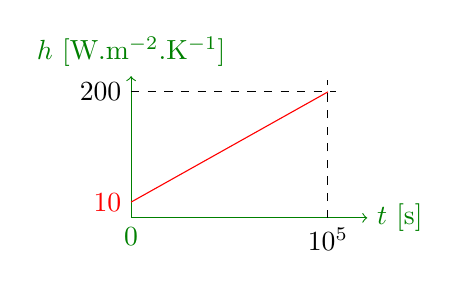
\begin{tikzpicture}
            \draw [<->,Green] (0,1.8) node (yaxis) [above] {$h$ [W.m$^{-2}$.K$^{-1}$]}
                           |- (3,0) node (xaxis) [right] {$t$ [s]};
            \draw [-,red] (0,0.2) node (hmin) [left] {\green{10}} -- (2.5,1.6);
            \draw[dashed] (0,1.6) node (hmax) [left] {\green{200}} -- (2.6,1.6) ;
            \draw[Green] (0,0) node[anchor=north] {0};
            \draw[dashed] (2.5,0) node (tmax) [below] {\green{10$^5$}} -- (2.5,1.75) ;
          \end{tikzpicture}
        \end{textblock*}
      \item<3-> \fe{\green{Conductivité fonction de la température}}
                   {\green{Temperature-dependent conductivity}}\\
                \green{$\lambda (T)=0.3T+200$}
      \item<4-> \fe{\green{Source fonction de la température}}
                   {\green{Temperature-dependent heat source}}\\
                \green{$q(T)=4.10^6~\tx{exp}^{-\left(\frac{T-1000}{700}\right)^2}$}
      \begin{center}
        \fe{\avous{~À vous de jouer !}}{\avous{~It's up to you!}}
      \end{center}
    \end{enumerate}
  \end{itemize}
\end{frame}
}

{\setbeamerfont{framesubtitle}{size=\tiny}
\begin{frame}{\fe{Exercice 3 : dépendance à la température}
                 {Exercise 3: temperature-dependence}}
             {\url{https://www-cast3m.cea.fr/index.php?page=exemples&exemple=formation_pasapas_3_initial}}
  \begin{itemize}
    \item \fe{Quelques objets utiles}{Some useful objects}\\
    \footnotesize
    \kw{sou~~} \fe{maillage de la source de chaleur}{heat source mesh}\\
    \kw{mosou} \fe{modèle thermique réduit sur le maillage de la source}{reduced thermal model on the heat source mesh}\\
    \normalsize
    \item \fe{Quelques opérateurs utiles}{Some useful operators}\\
    \footnotesize
    \kwr{REDU} \fe{réduction des températures sur \kw{sou}}{reduce temperatures on \kw{sou}}\\
    \kwr{SOUR} \fe{imposer une source volumique de chaleur}{impose a volume heat source}\\
    \normalsize
    \item \fe{Quelques indices utiles de la table}{Some useful table indices}\\
    \footnotesize
    \kwg{'WTABLE'.'THER\_COURANT'} \fe{températures courantes (itérations de \kwo{TRANSNON})}
                                      {current temperatures (\kwo{TRANSNON} iterations)}\\
    \kwg{'WTABLE'.'CHARGEMENT'} \fe{chargement courant}{current load}
    \normalsize
  \end{itemize}
\end{frame}
}
